\section{Résultats obtenus}
\label{sec:resultats}

Sauf mention contraire, tous les résultats de cette section sont mesurés sur l'ensemble de test (344 images), qui n'a servi à aucun choix, et donnés sous la forme moyenne $\pm$ écart-type sur les cinq modèles issus de la validation croisée.

\subsection{Caractéristiques de l'unité de calcul}
\label{sec:materiel}

Toutes les expériences ont été menées sur un ordinateur portable dont le tableau~\ref{tab:hardware} décrit la configuration. Les entraînements ont été lancés les uns après les autres, jamais en parallèle, pour que les temps mesurés restent comparables, et tous utilisent les hyperparamètres du tableau~\ref{tab:hyper}. Les 65 entraînements principaux ont demandé 2~h~43 de calcul au total.

\begin{table}[htbp]
\centering
\caption{Environnement matériel et logiciel.}
\label{tab:hardware}
\small
\begin{tabularx}{0.92\textwidth}{l X}
\toprule
\textbf{Composant} & \textbf{Caractéristiques} \\
\midrule
Processeur & AMD Ryzen 9 8945HX (16 cœurs, 32 threads) \\
Carte graphique & NVIDIA GeForce RTX 5070 Laptop GPU, 8~Go de mémoire (architecture Blackwell) \\
Mémoire vive & 32~Go \\
Système d'exploitation & Windows 11 Pro \\
Langage & Python 3.12.13 \\
Apprentissage profond & PyTorch 2.14.1 (CUDA 13.0, cuDNN 9.24), torchvision 0.29.1, timm 1.0.31 \\
Analyse et figures & scikit-learn 1.9.1, NumPy 2.5.4, pandas 3.1.1, Matplotlib 3.11.2 \\
\bottomrule
\end{tabularx}
\end{table}

\subsection{Courbes d'apprentissage}
\label{sec:courbes}

La figure~\ref{fig:lc-fft} montre l'évolution de l'accuracy et de la perte au fil des époques en fine-tuning complet, en moyenne sur les cinq plis (la bande colorée correspond à $\pm$ un écart-type). Les quatre réseaux pré-entraînés convergent très vite : l'accuracy de validation dépasse 90\,\% dès la deuxième ou la troisième époque, et même dès la première pour ConvNeXtV2, puis se stabilise entre 97 et 99\,\% après une dizaine d'époques. L'accuracy d'apprentissage atteint presque 100\,\% et la perte d'apprentissage passe sous la perte de validation à partir de la cinquième époque environ. Il y a donc un léger surapprentissage, mais la perte de validation ne remonte jamais : la régularisation (augmentation, dropout, lissage des étiquettes, taux d'apprentissage réduit pour les couches pré-entraînées) suffit à le contenir. La perte ne descend pas sous 0,4 environ ; c'est l'effet attendu du lissage des étiquettes, qui empêche le modèle de viser une probabilité de 1.

Le CNN entraîné from scratch se comporte tout autrement. Il démarre autour de 50\,\%, progresse lentement et régulièrement, et atteint 94\,\% à la dernière époque, sans que l'écart entre apprentissage et validation ne se creuse. Ses courbes ne sont pas stabilisées après 30 époques : ce modèle souffre plutôt de sous-apprentissage et gagnerait sans doute quelques points avec un entraînement plus long. Nous avons préféré garder des conditions identiques pour tous les modèles, mais il faut garder cette limite en tête en lisant les comparaisons. Ses bandes d'écart-type, plus larges, traduisent aussi une plus grande sensibilité au pli.

\begin{figure}[htbp]
\centering
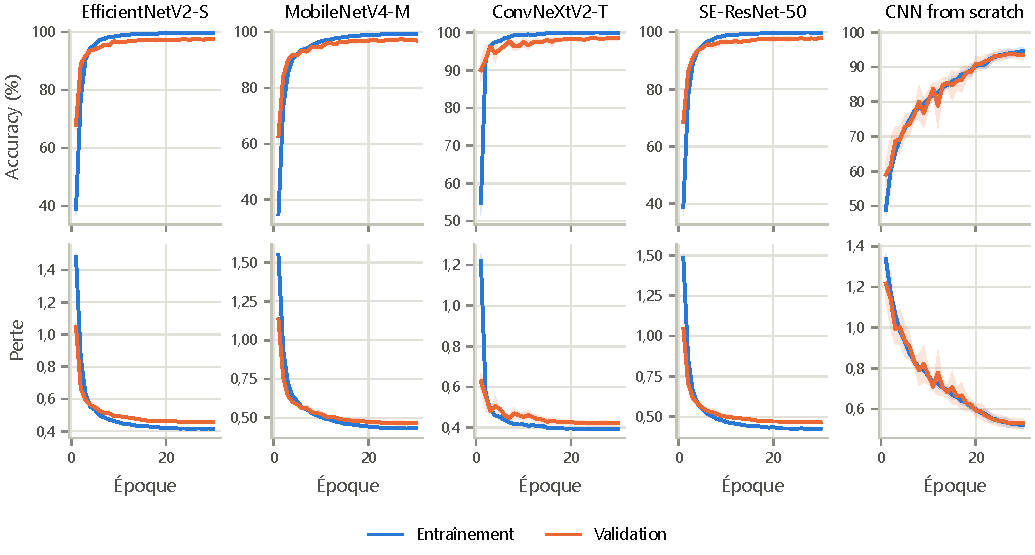
\includegraphics[width=\textwidth]{learning_curves_full_finetuning.pdf}
\caption{Courbes d'apprentissage en fine-tuning complet et pour le CNN from scratch (moyenne sur 5 plis, bande : $\pm$ un écart-type).}
\label{fig:lc-fft}
\end{figure}

En extraction de caractéristiques (figure~\ref{fig:lc-fe}), les courbes plafonnent bien plus bas, entre 84\,\% (MobileNetV4) et 91\,\% (EfficientNetV2-S, ConvNeXtV2 et SE-ResNet-50) en validation, et ce plafond est atteint vers la quinzième époque. La perte reste élevée, entre 0,6 et 0,75. Avec un réseau gelé, le modèle ne peut apprendre qu'une frontière linéaire dans l'espace des embeddings ImageNet, et cet espace sépare manifestement moins bien nos cinq classes. Le fine-tuning partiel (figure~\ref{fig:lc-pft}) a des courbes proches de celles du fine-tuning complet, avec un plateau un peu plus bas.

\begin{figure}[htbp]
\centering
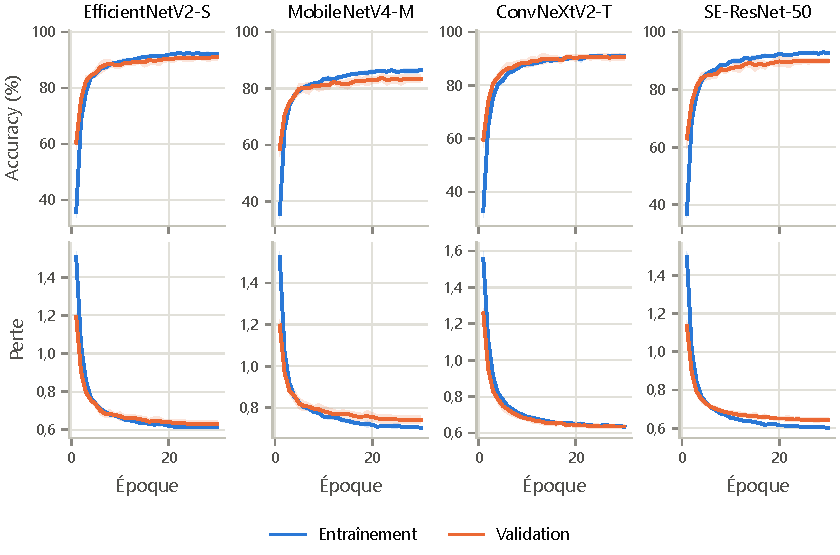
\includegraphics[width=0.9\textwidth]{learning_curves_feature_extraction.pdf}
\caption{Courbes d'apprentissage en extraction de caractéristiques (moyenne sur 5 plis).}
\label{fig:lc-fe}
\end{figure}

\begin{figure}[htbp]
\centering
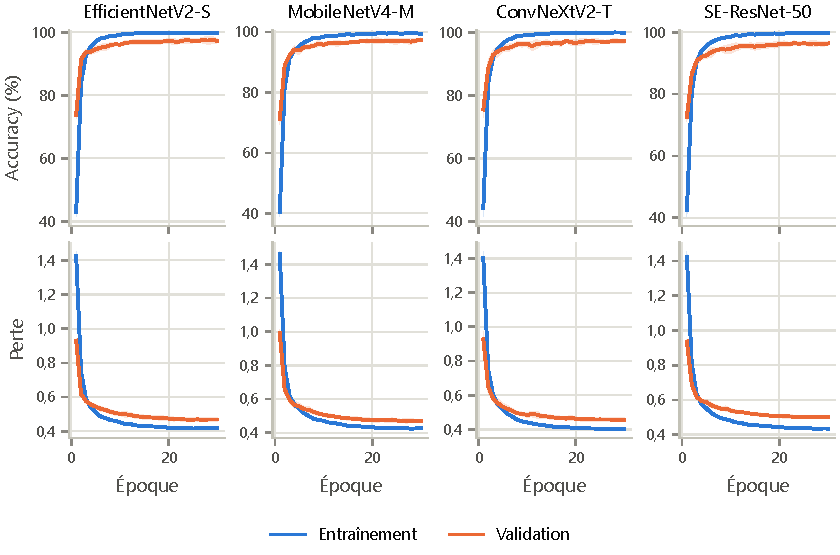
\includegraphics[width=0.9\textwidth]{learning_curves_partial_finetuning.pdf}
\caption{Courbes d'apprentissage en fine-tuning partiel (moyenne sur 5 plis).}
\label{fig:lc-pft}
\end{figure}

\subsection{Matrices de confusion}
\label{sec:confusion}

La figure~\ref{fig:confusion} présente les matrices de confusion des modèles en fine-tuning complet, du CNN from scratch et du modèle de fusion. Chacune cumule les prédictions des cinq modèles de la validation croisée sur l'ensemble de test (soit 1\,720 prédictions) et est normalisée par ligne : la diagonale donne le rappel de chaque classe, en pourcentage.

\begin{figure}[htbp]
\centering
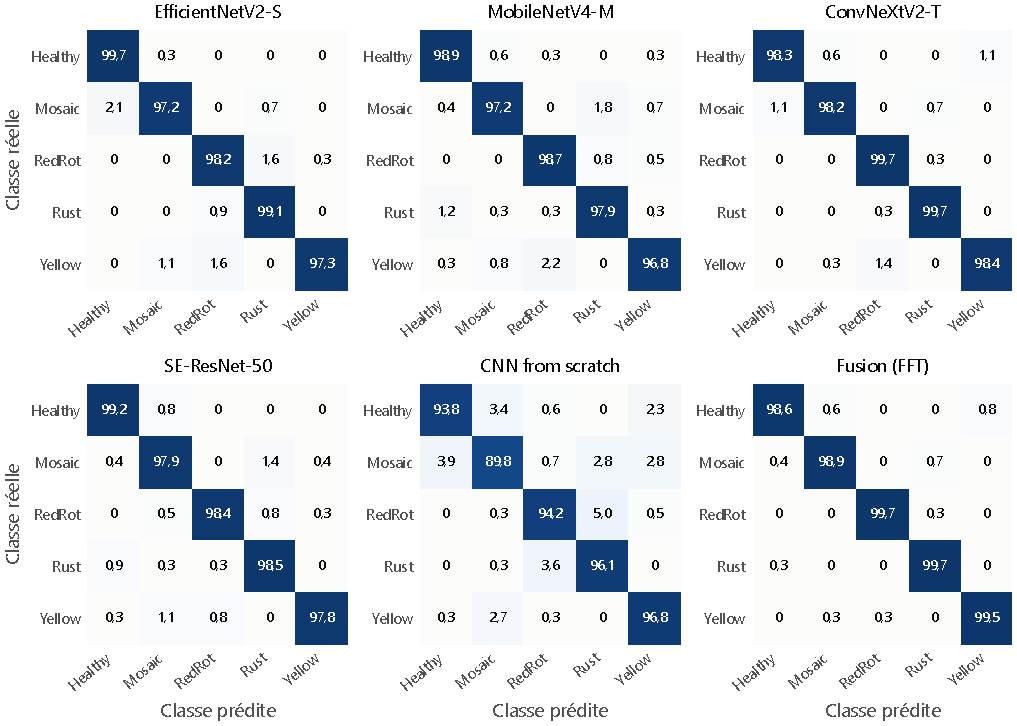
\includegraphics[width=\textwidth]{confusion_matrices.pdf}
\caption{Matrices de confusion normalisées par ligne (en \%), cumulées sur les cinq plis.}
\label{fig:confusion}
\end{figure}

Les erreurs des modèles pré-entraînés sont rares et se concentrent sur quelques paires de classes. Mosaic est la classe la plus difficile pour presque tous : son rappel varie de 97,2 à 98,2\,\% en fine-tuning complet et tombe à 89,8\,\% pour le CNN from scratch. Ses symptômes, des marbrures vert clair souvent discrètes, peuvent passer pour une feuille saine légèrement décolorée, d'où les confusions Mosaic $\rightarrow$ Healthy (2,1\,\% pour EfficientNetV2-S). C'est aussi la classe la plus réduite après nettoyage, avec 376 images. Deux autres confusions reviennent d'un modèle à l'autre : RedRot et Rust, qui présentent toutes deux des lésions brun-rouge allongées, et Yellow $\rightarrow$ RedRot (jusqu'à 2,2\,\% pour MobileNetV4), deux maladies qui modifient la couleur de la nervure centrale. Le CNN from scratch commet les mêmes types d'erreurs, mais bien plus souvent : 5,0\,\% des feuilles atteintes de pourriture rouge sont classées comme rouillées et 3,9\,\% des feuilles atteintes de mosaïque comme saines. Enfin, la fusion des embeddings fine-tunés (dernière matrice) réduit encore les confusions des modèles seuls : le rappel de Mosaic monte à 98,9\,\% et celui de Yellow à 99,5\,\%.

\subsection{Courbes ROC}
\label{sec:roc}

Les courbes ROC \og une classe contre toutes \fg{} (figure~\ref{fig:roc}) collent au coin supérieur gauche pour tous les modèles pré-entraînés ; il faut l'agrandissement de la région $\mathrm{FPR} \le 0{,}06$ pour voir des différences. On y retrouve la hiérarchie de la matrice de confusion : la courbe de la classe Mosaic est presque toujours la plus basse, et celles du CNN from scratch s'écartent nettement des autres.

\begin{figure}[htbp]
\centering
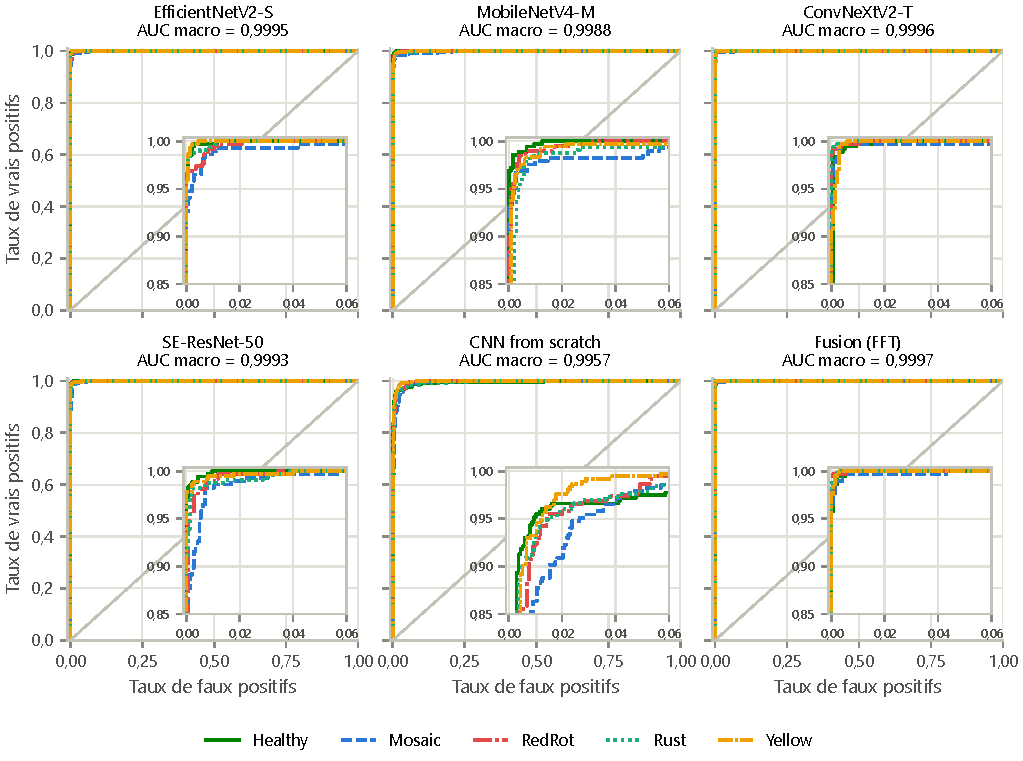
\includegraphics[width=\textwidth]{roc_curves.pdf}
\caption{Courbes ROC une classe contre toutes, calculées sur les prédictions cumulées des cinq plis. L'encart agrandit la région des faibles taux de faux positifs.}
\label{fig:roc}
\end{figure}

\subsection{AUC}
\label{sec:auc}

Le tableau~\ref{tab:auc} donne l'aire sous la courbe ROC pour chaque classe. Toutes les valeurs des modèles pré-entraînés dépassent 0,998, et la plupart 0,999 : lorsque ces modèles se trompent, ce n'est presque jamais avec assurance, puisque la bonne classe reçoit tout de même un score élevé. Même le CNN from scratch atteint 0,995 sur chaque classe, alors que son accuracy n'est que de 94\,\%. L'AUC est donc ici peu discriminante, et c'est surtout l'accuracy et le F1-score qui permettent de départager les modèles.

\begin{table}[htbp]
\centering
\caption{AUC par classe (une contre toutes), calculée sur les prédictions cumulées des cinq plis. En gras : meilleure valeur de chaque ligne.}
\label{tab:auc}
\small
\resizebox{\textwidth}{!}{%
\begin{tabular}{lccccccc}
\toprule
\textbf{Classe} & \textbf{EffNetV2-S} & \textbf{MNv4-M} & \textbf{ConvNeXtV2-T} & \textbf{SE-ResNet-50} & \textbf{Scratch} & \textbf{Fusion (FFT)} & \textbf{Vote souple} \\
\midrule
\tableinput{tables/results_per_class_auc.tex}
\bottomrule
\end{tabular}%
}
\end{table}

\subsection{Résultats globaux}
\label{sec:globaux}

Le tableau~\ref{tab:main} reprend le format demandé par l'énoncé, pour la meilleure stratégie de chaque architecture, le fine-tuning complet, ainsi que pour le CNN from scratch et les deux formes de fusion. Le tableau~\ref{tab:strategies} détaille ensuite les trois stratégies de transfert.

\begin{table}[htbp]
\centering
\caption{Résultats globaux sur l'ensemble de test (moyenne $\pm$ écart-type sur 5 plis). Précision, rappel et F1 sont des moyennes macro. Le temps est celui d'un entraînement complet (30 époques, validation comprise). $^{*}$ Pour les fusions, le nombre de paramètres et le temps incluent les quatre réseaux fine-tunés.}
\label{tab:main}
\small
\setlength{\tabcolsep}{4pt}
\resizebox{\textwidth}{!}{%
\begin{tabular}{lccccccc}
\toprule
\textbf{Modèle} & \textbf{Accuracy (\%)} & \textbf{Précision (\%)} & \textbf{Rappel (\%)} & \textbf{F1 (\%)} & \textbf{AUC} & \makecell{\textbf{Param.}\\\textbf{(M)}} & \makecell{\textbf{Temps}\\\textbf{d'entraîn.}} \\
\midrule
\tableinput{tables/results_main.tex}
\bottomrule
\end{tabular}%
}
\end{table}

\begin{table}[htbp]
\centering
\caption{Comparaison des stratégies de transfert. Accuracy de validation (pli de validation, utilisé pour choisir l'époque) et métriques de test. La mémoire est le pic d'occupation GPU pendant l'entraînement.}
\label{tab:strategies}
\footnotesize
\setlength{\tabcolsep}{3.5pt}
\resizebox{\textwidth}{!}{%
\begin{tabular}{llccccccc}
\toprule
\textbf{Modèle} & \textbf{Stratégie} & \makecell{\textbf{Param.}\\\textbf{entraînables}} & \makecell{\textbf{Acc. val.}\\\textbf{(\%)}} & \makecell{\textbf{Acc. test}\\\textbf{(\%)}} & \makecell{\textbf{F1 test}\\\textbf{(\%)}} & \textbf{AUC test} & \textbf{Temps} & \makecell{\textbf{Mémoire}\\\textbf{(Go)}} \\
\midrule
\tableinput{tables/results_strategies.tex}
\bottomrule
\end{tabular}%
}
\end{table}

Plusieurs enseignements ressortent de ces deux tableaux.

\paragraph{Le fine-tuning complet l'emporte pour toutes les architectures.} Avec $98{,}9 \pm 0{,}6$\,\% d'accuracy, ConvNeXtV2-T obtient le meilleur résultat, devant SE-ResNet-50 (98,4\,\%), EfficientNetV2-S (98,3\,\%) et MobileNetV4-M (97,9\,\%). Les quatre modèles tiennent en un point, un écart du même ordre que la variation d'un pli à l'autre (0,4 à 0,8 point). Pour savoir si ces différences sont réelles, nous avons estimé par bootstrap, avec 10\,000 rééchantillonnages des images de test, un intervalle de confiance à 95\,\% de l'écart avec le meilleur modèle (tableau~\ref{tab:significance}). Seuls MobileNetV4 ($-1{,}0$ point) et le CNN from scratch ($-4{,}6$ points) sont significativement en dessous de ConvNeXtV2 ; l'avance de ce dernier sur EfficientNetV2-S et SE-ResNet-50 n'est pas significative avec 344 images de test.

\begin{table}[htbp]
\centering
\caption{Accuracy de test et intervalle de confiance à 95\,\% obtenu par bootstrap sur les images de test (10\,000 tirages). L'écart est mesuré par rapport au meilleur modèle unique, ConvNeXtV2-T (une valeur positive signifie que le modèle fait mieux que lui) ; il est jugé significatif si son intervalle de confiance exclut zéro.}
\label{tab:significance}
\small
\resizebox{\textwidth}{!}{%
\begin{tabular}{lccccc}
\toprule
\textbf{Modèle} & \textbf{Accuracy (\%)} & \textbf{IC 95\,\%} & \makecell{\textbf{Écart avec}\\\textbf{ConvNeXtV2-T (points)}} & \textbf{IC 95\,\% de l'écart} & \textbf{Significatif} \\
\midrule
\tableinput{tables/results_significance.tex}
\bottomrule
\end{tabular}%
}
\end{table}

\paragraph{Le niveau de fine-tuning compte davantage que l'architecture.} Passer de l'extraction de caractéristiques au fine-tuning complet fait gagner entre 7,6 points (SE-ResNet-50) et 14,0 points (MobileNetV4), alors que les quatre architectures ne diffèrent que d'un point une fois fine-tunées (figure~\ref{fig:strategies}). Le fine-tuning partiel se place entre les deux. Il récupère l'essentiel du gain pour EfficientNetV2-S (97,2\,\%), mais reste 3,4 points sous le fine-tuning complet pour ConvNeXtV2 (95,5\,\%), alors qu'il entraîne déjà 56\,\% de ses paramètres. Ré-entraîner le seul dernier étage ne suffit donc pas : les étages intermédiaires, qui encodent des textures et des motifs de taille moyenne, doivent eux aussi s'adapter à des lésions foliaires très différentes des objets d'ImageNet. Le fine-tuning partiel garde en revanche l'avantage du coût : pour ConvNeXtV2, il prend 2~minutes au lieu de 5 et occupe 0,83~Go de mémoire GPU au lieu de 3,85.

\begin{figure}[htbp]
\centering
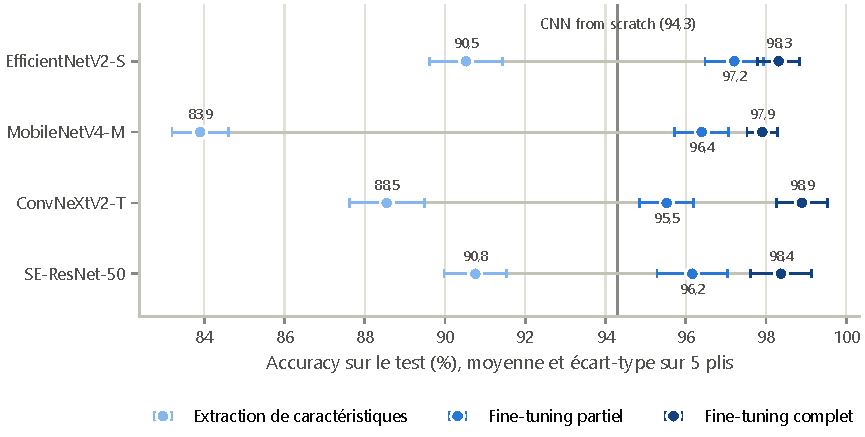
\includegraphics[width=0.9\textwidth]{strategy_comparison.pdf}
\caption{Accuracy de test selon la stratégie de transfert (moyenne et écart-type sur 5 plis). La ligne verticale grise indique le CNN entraîné from scratch.}
\label{fig:strategies}
\end{figure}

\paragraph{Un petit CNN from scratch fait mieux que l'extraction de caractéristiques.} Résultat plus inattendu, notre CNN de 1,2 million de paramètres (94,3\,\%) dépasse toutes les variantes en extraction de caractéristiques (83,9 à 90,8\,\%). Les caractéristiques ImageNet gelées, apprises pour distinguer des chiens, des voitures ou des oiseaux, ne séparent pas linéairement des différences aussi fines que celles qui distinguent une feuille saine d'une feuille atteinte de mosaïque ; un réseau, même modeste, qui adapte toutes ses couches à la tâche s'en sort mieux. Le transfert redevient nettement gagnant dès qu'on autorise le fine-tuning : avec ConvNeXtV2, le taux d'erreur passe de 5,7\,\% à 1,1\,\%, soit cinq fois moins d'erreurs, et le modèle est beaucoup plus stable d'un pli à l'autre (écart-type de 0,6 point contre 2,1).

\paragraph{La validation est un peu optimiste pour les stratégies partielles.} En fine-tuning complet, l'accuracy de validation et celle de test sont très proches. En extraction de caractéristiques et en fine-tuning partiel, la validation surestime parfois le test, jusqu'à 2,6 points pour ConvNeXtV2. L'époque retenue étant choisie sur le pli de validation, cette mesure est légèrement biaisée vers le haut ; c'est précisément pour cela qu'il fallait un ensemble de test qui n'intervienne dans aucun choix.

\paragraph{Performances par maladie.} Le tableau~\ref{tab:perclass} donne le F1-score de chaque classe. En fine-tuning complet, toutes les classes dépassent 97\,\% pour les quatre réseaux, et ConvNeXtV2 dépasse 98,5\,\% sur les cinq. Mosaic reste la classe la plus faible pour la plupart des modèles, et l'écart avec les autres classes se creuse fortement pour le CNN from scratch (90,6\,\%).

\begin{table}[htbp]
\centering
\caption{F1-score par classe (en \%), calculé sur les prédictions cumulées des cinq plis. En gras : meilleure valeur de chaque ligne.}
\label{tab:perclass}
\small
\resizebox{\textwidth}{!}{%
\begin{tabular}{lccccccc}
\toprule
\textbf{Classe} & \textbf{EffNetV2-S} & \textbf{MNv4-M} & \textbf{ConvNeXtV2-T} & \textbf{SE-ResNet-50} & \textbf{Scratch} & \textbf{Fusion (FFT)} & \textbf{Vote souple} \\
\midrule
\tableinput{tables/results_per_class_f1.tex}
\bottomrule
\end{tabular}%
}
\end{table}

\subsection{Fusion de caractéristiques}
\label{sec:resultats-fusion}

Le tableau~\ref{tab:fusion} et la figure~\ref{fig:fusion} présentent la fusion des embeddings pour les 15 combinaisons possibles des quatre réseaux, à partir des réseaux gelés (embeddings ImageNet) et des réseaux issus du fine-tuning complet. Dans les deux cas, seule la tête de fusion est entraînée, sur des embeddings extraits une fois pour toutes, sans augmentation. Les lignes à un seul réseau servent de référence dans ce même protocole ; pour les embeddings ImageNet, elles retrouvent à un point près les résultats de l'extraction de caractéristiques du tableau~\ref{tab:strategies}, ce qui montre que l'absence d'augmentation ne change pas les conclusions.

\begin{table}[htbp]
\centering
\caption{Fusion des embeddings (accuracy et F1 de test, en \%, moyenne $\pm$ écart-type sur 5 plis). E : EfficientNetV2-S, M : MobileNetV4-M, C : ConvNeXtV2-T, S : SE-ResNet-50. La dernière ligne donne le vote souple des quatre modèles fine-tunés. En gras : meilleure accuracy de chaque colonne.}
\label{tab:fusion}
\small
\begin{tabular}{clcccc}
\toprule
& & \multicolumn{2}{c}{\textbf{Embeddings ImageNet (gelés)}} & \multicolumn{2}{c}{\textbf{Embeddings fine-tunés}} \\
\cmidrule(lr){3-4}\cmidrule(lr){5-6}
\textbf{$M$} & \textbf{Réseaux fusionnés} & \textbf{Accuracy} & \textbf{F1} & \textbf{Accuracy} & \textbf{F1} \\
\midrule
\tableinput{tables/results_fusion.tex}
\bottomrule
\end{tabular}
\end{table}

\paragraph{Sur des réseaux gelés, la fusion aide sans remplacer le fine-tuning.} Avec les embeddings ImageNet, le meilleur réseau seul (EfficientNetV2-S, 91,1\,\%) est dépassé par la fusion des quatre, qui atteint $92{,}7 \pm 0{,}5$\,\%, soit 1,6 point de mieux avec un écart-type deux fois plus faible. Le gain plafonne dès trois réseaux. Détail intéressant, MobileNetV4, le plus faible seul (84,1\,\%), fait partie de l'un des deux meilleurs triplets (M + C + S) : ses représentations, bien que moins discriminantes, apportent une information que les autres n'ont pas. Mais même la meilleure fusion de réseaux gelés reste cinq points en dessous du moins bon modèle fine-tuné : juxtaposer plusieurs représentations génériques ne remplace pas l'adaptation des réseaux au domaine.

\paragraph{Sur des réseaux fine-tunés, la fusion donne le meilleur résultat de l'étude.} Les embeddings issus du fine-tuning complet sont déjà très discriminants : une simple tête linéaire réentraînée dessus retrouve les performances des modèles d'origine (99,0\,\% pour ConvNeXtV2). La fusion les améliore encore : 99,1\,\% pour les meilleures paires, 99,2\,\% pour le meilleur triplet et $99{,}3 \pm 0{,}6$\,\% pour les quatre réseaux. Le vote souple des quatre modèles fine-tunés, qui ne demande aucun apprentissage supplémentaire, fait aussi bien ($99{,}4 \pm 0{,}5$\,\%) ; la différence entre les deux fusions n'est pas significative. Toutes deux réduisent d'environ moitié le taux d'erreur du meilleur modèle seul, qui passe de 1,1\,\% à 0,6\,\%, et leur avance sur ConvNeXtV2 (+0,4 et +0,5 point) est significative dans les deux cas (tableau~\ref{tab:significance}).

\begin{figure}[htbp]
\centering
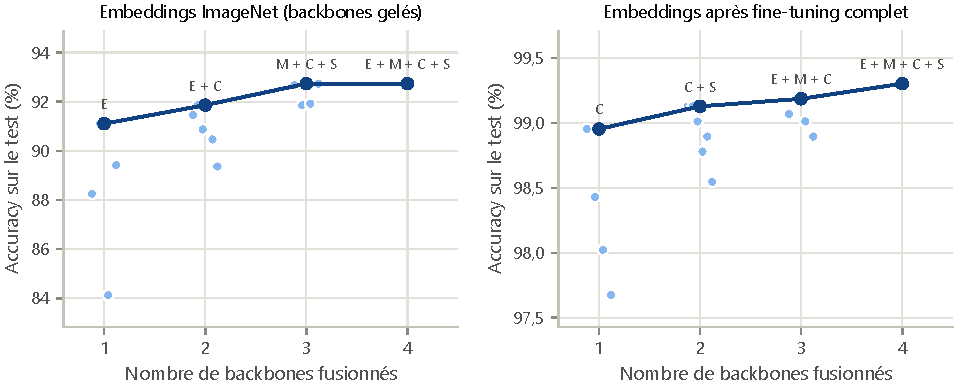
\includegraphics[width=0.95\textwidth]{fusion_gain.pdf}
\caption{Accuracy de test selon le nombre de réseaux fusionnés. Chaque point clair est une combinaison ; la ligne foncée relie la meilleure combinaison de chaque taille.}
\label{fig:fusion}
\end{figure}

Ce gain a un prix. La fusion des quatre réseaux mobilise 82,6 millions de paramètres et environ 24,4~GFLOPs par image, soit trois fois plus que ConvNeXtV2 seul, et suppose d'entraîner quatre modèles. Elle se justifie pour un service d'analyse centralisé, où chaque erreur évitée compte ; elle se justifie beaucoup moins sur un téléphone.

\subsection{Analyse comparative}
\label{sec:analyse}

\subsubsection{Quel modèle est le plus précis ?}
\label{sec:precision}

Parmi les modèles uniques, ConvNeXtV2-T en fine-tuning complet est le plus précis, avec $98{,}9 \pm 0{,}6$\,\% d'accuracy et un F1 macro de 98,9\,\%, mais son avance sur SE-ResNet-50 et EfficientNetV2-S n'est pas significative. Les deux fusions font mieux encore (99,3 et 99,4\,\%) et sont les seules à battre ConvNeXtV2 de façon significative. Pour la précision pure, sans contrainte de calcul, il faut donc retenir le vote souple des quatre modèles fine-tunés ; pour un modèle unique, ConvNeXtV2-T. Notons que le classement ne suit pas celui d'ImageNet : EfficientNetV2-S, le meilleur des quatre sur ImageNet (tableau~\ref{tab:models}), n'est que troisième ici, ce qui rappelle qu'avec quatre modèles seulement et des écarts aussi faibles, la corrélation observée par Kornblith et al. \cite{kornblith2019better} ne peut pas servir de règle de choix.

\subsubsection{Quel modèle est le plus léger ?}
\label{sec:legerete}

Le tableau~\ref{tab:efficiency} et la figure~\ref{fig:efficiency} comparent le coût des modèles en inférence. MobileNetV4-M est de loin le plus léger des réseaux pré-entraînés : 8,4 millions de paramètres (32~Mo en float32) et 1,65~GFLOPs par image, soit trois à cinq fois moins que les autres. Sur le processeur, il classe une image en 30~ms, contre 64 à 97~ms pour les autres réseaux, et c'est aussi le plus rapide à entraîner (2~min~21~s par pli) et le moins gourmand en mémoire GPU (0,94~Go). Il ne perd qu'un point d'accuracy par rapport à ConvNeXtV2 (97,9 contre 98,9\,\%), ce qui en fait le meilleur candidat pour une application sur téléphone.

\begin{table}[htbp]
\centering
\caption{Coût des modèles en inférence (entrée $224\times224$). Latence mesurée image par image (lot de 1), sur GPU en bfloat16 et sur CPU en float32 avec 4 threads ; débit mesuré sur GPU avec des lots de 32 images.}
\label{tab:efficiency}
\small
\begin{tabular}{lcccccc}
\toprule
\textbf{Modèle} & \makecell{\textbf{Paramètres}\\\textbf{(M)}} & \makecell{\textbf{Taille}\\\textbf{(Mo)}} & \textbf{GFLOPs} & \makecell{\textbf{Latence}\\\textbf{GPU (ms)}} & \makecell{\textbf{Débit GPU}\\\textbf{(images/s)}} & \makecell{\textbf{Latence}\\\textbf{CPU (ms)}} \\
\midrule
\tableinput{tables/results_efficiency.tex}
\bottomrule
\end{tabular}
\end{table}

Sur GPU, la hiérarchie est différente et mérite une remarque. Avec une seule image à la fois, la carte graphique est loin d'être saturée et la latence dépend surtout du nombre d'opérations à lancer les unes après les autres : ConvNeXtV2, avec ses 18 blocs, répond le plus vite (17~ms), alors qu'EfficientNetV2-S et ses 40 blocs, plus légers mais plus nombreux, mettent 50~ms. Dès que l'on traite des lots, le nombre d'opérations reprend le dessus et MobileNetV4 traite 1\,673 images par seconde, 2,6 fois plus que ConvNeXtV2. Le CNN from scratch est encore plus léger (1,2 million de paramètres, 12~ms sur CPU), mais il paie cette légèreté de près de cinq points d'accuracy. À l'autre extrémité, la fusion des quatre réseaux coûte environ trois fois plus que ConvNeXtV2 seul pour un demi-point de gain.

\begin{figure}[htbp]
\centering
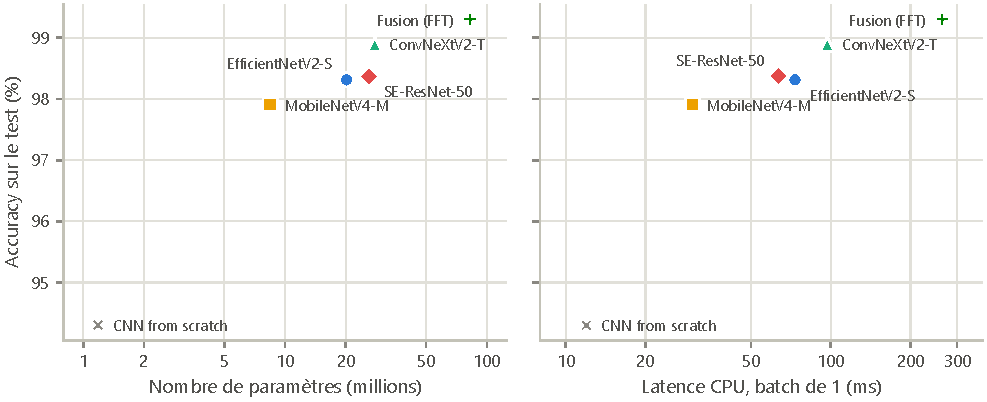
\includegraphics[width=\textwidth]{efficiency_tradeoff.pdf}
\caption{Compromis entre accuracy de test et coût d'inférence (axes horizontaux logarithmiques).}
\label{fig:efficiency}
\end{figure}

\subsubsection{Quel modèle est le plus robuste ?}
\label{sec:robustesse}

Une photo prise au champ avec un téléphone d'entrée de gamme est rarement parfaite : bruit de capteur en faible lumière, flou de bougé, sous-exposition, compression agressive à l'envoi, feuille partiellement masquée. Pour mesurer la robustesse des modèles à ces défauts, nous avons dégradé l'ensemble de test de cinq façons, à trois niveaux de sévérité, sans jamais montrer ces dégradations aux modèles pendant l'apprentissage : bruit gaussien d'écart-type $\sigma \in \{0{,}04 ; 0{,}08 ; 0{,}12\}$, flou gaussien ($\sigma \in \{1 ; 2 ; 3\}$ pixels), assombrissement (intensités multipliées par 0,7, 0,5 ou 0,3), compression JPEG (qualité 30, 15 ou 5) et occultation par un carré gris couvrant 25, 35 ou 45\,\% du côté de l'image, placé au hasard. La figure~\ref{fig:robustness} et le tableau~\ref{tab:robustness} donnent les résultats.

\begin{figure}[htbp]
\centering
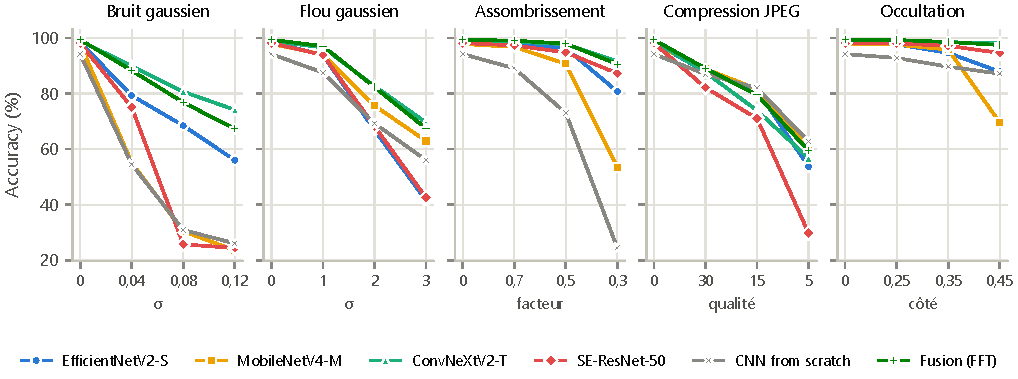
\includegraphics[width=\textwidth]{robustness.pdf}
\caption{Accuracy de test en fonction de la sévérité de la dégradation (moyenne sur 5 plis). Le niveau 0 correspond aux images d'origine.}
\label{fig:robustness}
\end{figure}

\begin{table}[htbp]
\centering
\caption{Robustesse aux dégradations : accuracy (en \%) sur les images d'origine, puis moyenne sur les trois niveaux de chaque dégradation, moyenne générale et baisse par rapport aux images d'origine. La colonne \og Original \fg{} est recalculée dans le même protocole (images requantifiées sur 8 bits), d'où de légers écarts avec le tableau~\ref{tab:main}.}
\label{tab:robustness}
\small
\setlength{\tabcolsep}{4.5pt}
\resizebox{\textwidth}{!}{%
\begin{tabular}{lcccccccc}
\toprule
\textbf{Modèle} & \textbf{Original} & \textbf{Bruit} & \textbf{Flou} & \makecell{\textbf{Assom-}\\\textbf{brissement}} & \textbf{JPEG} & \textbf{Occultation} & \textbf{Moyenne} & \textbf{Baisse} \\
\midrule
\tableinput{tables/results_robustness.tex}
\bottomrule
\end{tabular}%
}
\end{table}

Le constat principal est une grande disparité entre architectures, que l'accuracy sur images propres ne laissait pas deviner. Les quatre réseaux fine-tunés sont à moins d'un point les uns des autres sur les images d'origine, mais leur accuracy moyenne sur images dégradées va de 71,7\,\% (MobileNetV4) à 86,4\,\% (ConvNeXtV2). Le bruit gaussien est la dégradation la plus discriminante : au niveau le plus fort, ConvNeXtV2 conserve 74\,\% d'accuracy, alors que MobileNetV4 et SE-ResNet-50 tombent sous 25\,\%, à peine mieux que le hasard (20\,\%). Une forte compression JPEG (qualité 5) pénalise tous les modèles, tandis que l'occultation d'une partie de la feuille est bien tolérée, sauf au niveau le plus fort par MobileNetV4 (69,5\,\%) et, dans une moindre mesure, par EfficientNetV2-S (87,8\,\%). Le CNN from scratch est le plus fragile de tous (67,5\,\% en moyenne), en particulier face au bruit et à l'assombrissement.

Un second constat nous a surpris. Pour trois architectures sur quatre, le fine-tuning partiel est nettement plus robuste que le fine-tuning complet, alors qu'il est moins précis sur images propres : 81,2 contre 71,7\,\% en moyenne pour MobileNetV4, 80,6 contre 72,1\,\% pour SE-ResNet-50 et 83,6 contre 78,9\,\% pour EfficientNetV2-S. Une explication plausible est qu'en ré-entraînant tout le réseau sur des images propres, on spécialise aussi ses premiers filtres, ceux qui, appris sur la diversité d'ImageNet, étaient les plus tolérants au bruit ; en les gelant, le fine-tuning partiel conserve cette tolérance. ConvNeXtV2 fait exception : son fine-tuning complet est à la fois le plus précis et le plus robuste.

La réponse à la question posée est donc claire : parmi les modèles uniques, \textbf{ConvNeXtV2-T est le plus robuste}, avec la plus forte accuracy moyenne sous dégradation et la plus faible baisse (12,5 points). Le vote souple des quatre modèles fait encore un peu mieux (87,5\,\%, baisse de 11,9 points). La robustesse au changement de données d'apprentissage, mesurée par l'écart-type entre plis, départage moins les modèles : les quatre réseaux fine-tunés varient de 0,4 à 0,8 point d'un pli à l'autre, MobileNetV4 étant le plus régulier, alors que le CNN from scratch varie de 2,1 points.

\subsubsection{Quel est le besoin en données ?}
\label{sec:efficacite-donnees}

Pour vérifier que l'apprentissage par transfert réduit réellement le besoin en données, nous avons ré-entraîné ConvNeXtV2-T et MobileNetV4-M en fine-tuning complet, ainsi que le CNN from scratch, sur 10, 25 et 50\,\% des images d'apprentissage de chaque pli, tirées au hasard en respectant les proportions des classes. Les hyperparamètres, le pli de validation et l'ensemble de test sont inchangés. La figure~\ref{fig:data-efficiency} et le tableau~\ref{tab:data-efficiency} donnent les résultats.

\begin{figure}[htbp]
\centering
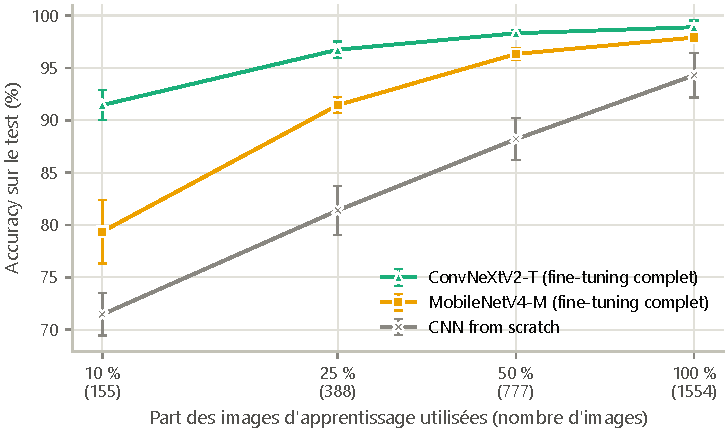
\includegraphics[width=0.8\textwidth]{data_efficiency.pdf}
\caption{Accuracy de test selon la part des images d'apprentissage utilisées (moyenne et écart-type sur 5 plis ; axe horizontal logarithmique). Entre parenthèses : nombre moyen d'images d'apprentissage par pli.}
\label{fig:data-efficiency}
\end{figure}

\begin{table}[htbp]
\centering
\caption{Accuracy de test (en \%) selon la part des images d'apprentissage utilisées, avec le nombre moyen d'images entre parenthèses (moyenne $\pm$ écart-type sur 5 plis).}
\label{tab:data-efficiency}
\small
\begin{tabular}{lcccc}
\toprule
\textbf{Modèle} & \textbf{10\,\% (155)} & \textbf{25\,\% (388)} & \textbf{50\,\% (777)} & \textbf{100\,\% (1\,554)} \\
\midrule
\tableinput{tables/results_data_efficiency.tex}
\bottomrule
\end{tabular}
\end{table}

L'avantage du pré-entraînement grandit à mesure que les données se raréfient. Avec seulement 155 images d'apprentissage, une trentaine par classe, ConvNeXtV2 reconnaît encore 91,5\,\% des images de test, alors que le CNN from scratch tombe à 71,5\,\% : vingt points d'écart, contre 4,6 avec toutes les données. Plus parlant encore, ConvNeXtV2 entraîné sur un quart des images (388) fait mieux (96,7\,\%) que le CNN from scratch entraîné sur la totalité (94,3\,\%), et avec la moitié des images il n'est plus qu'à 0,6 point de son score final. MobileNetV4 profite moins du pré-entraînement quand les données sont très rares (79,4\,\% avec 10\,\% des images, avec un écart-type de 3 points), ce qui suggère que ses représentations, plus compactes et optimisées pour la vitesse, se transfèrent moins bien avec très peu d'exemples ; l'écart avec ConvNeXtV2 se résorbe presque entièrement à partir de la moitié des données. Le CNN from scratch, enfin, progresse encore nettement entre 50 et 100\,\% des images : c'est lui qui profiterait le plus d'un jeu de données plus grand.
